\documentclass[10pt]{beamer}

\usepackage{settings}


\title{From Latent to Deep Latent}
\subtitle{Causal Inference with CEVAE}
\date{June 17, 2025}
\author[longname]{Valeria De Stasio, Christian Faccio, Giovanni Lucarelli}
\titlegraphic{\hfill
\includegraphics[height=1.3cm]{images/logo100_orizzontale.pdf}}

% add graphics path
\graphicspath{{../assets},{./images}}

\begin{document}

\maketitle

% magari un frame iniziale in cui introduciamo il concetto di causalità?
\begin{frame}{Objective: estimating causal effects}
    Estimate how a medical treatment $T$ affects the health $Y$ of a \textit{random} patient.

    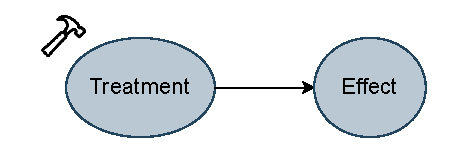
\includegraphics[width=\textwidth]{images/no_confounders.pdf}
  \begin{equation*}
    P(Y|\text{do}(T=t))=P(Y|T=t)
  \end{equation*}
  \begin{equation*}
    \text{ITE} = \mathbb{E}[(Y|\text{do}(T=1)]-\mathbb{E}[(Y|\text{do}(T=0)]
  \end{equation*}
  

\end{frame}


% How to intervene on already observed data?
\begin{frame}{Confounder}
  In a observational study we do \textbf{not} have control over 
  the treatment $T$: there may be a confounder $X$ that influences both variables!
  \begin{equation*}
    P(Y|\text{do}(T=t))\ne P(Y|T=t)
  \end{equation*}
    \begin{figure}
    \centering
    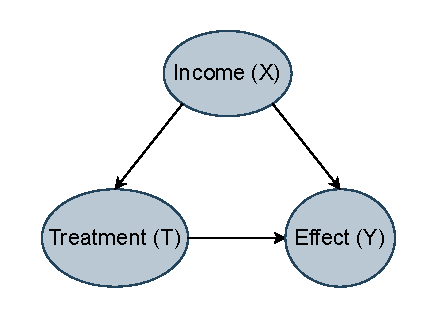
\includegraphics[width=0.5\textwidth]{images/unconfoundness.pdf}
  \end{figure}
  \begin{equation*}
    P(Y|\text{do}(T=t)) = \sum_{x} P(Y|T=t, X=x) P(X=x)
  \end{equation*}
\end{frame}

\begin{frame}{Latent confounder}
But what if there is a confounder $Z$ that is \textbf{not} observed?
    \begin{center}
  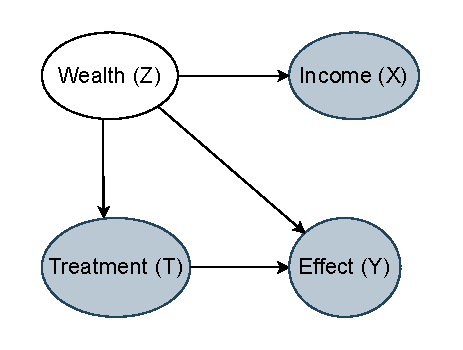
\includegraphics[width=0.5\textwidth]{images/latent_confounder.pdf}
\end{center}
  
We can use latent models:
\begin{itemize}
    \item Latent Variable Model
    \item Deep Latent Variable Model
\end{itemize} 
 \end{frame}

 \begin{frame}{Latent Variable Model}
     \begin{itemize}
         \item Assume parametric distributions
         \item Assume parametric relationships between variables
         \item Infer parameters using Stochastic Variational Inference (SVI)
         \item Problem: to infer from new data point $x$ we need to train a new model at test time! 
     \end{itemize}
 \end{frame}

  \begin{frame}{Deep Latent Variable Model}
     \begin{itemize}
         \item Assume parametric distributions
         \item Assume parametric relationships between variables through \alert{Neural Networks}
     \end{itemize}
 \end{frame}

\begin{frame}{Synthetic linear dataset}
    \begin{minipage}{0.48\textwidth}
      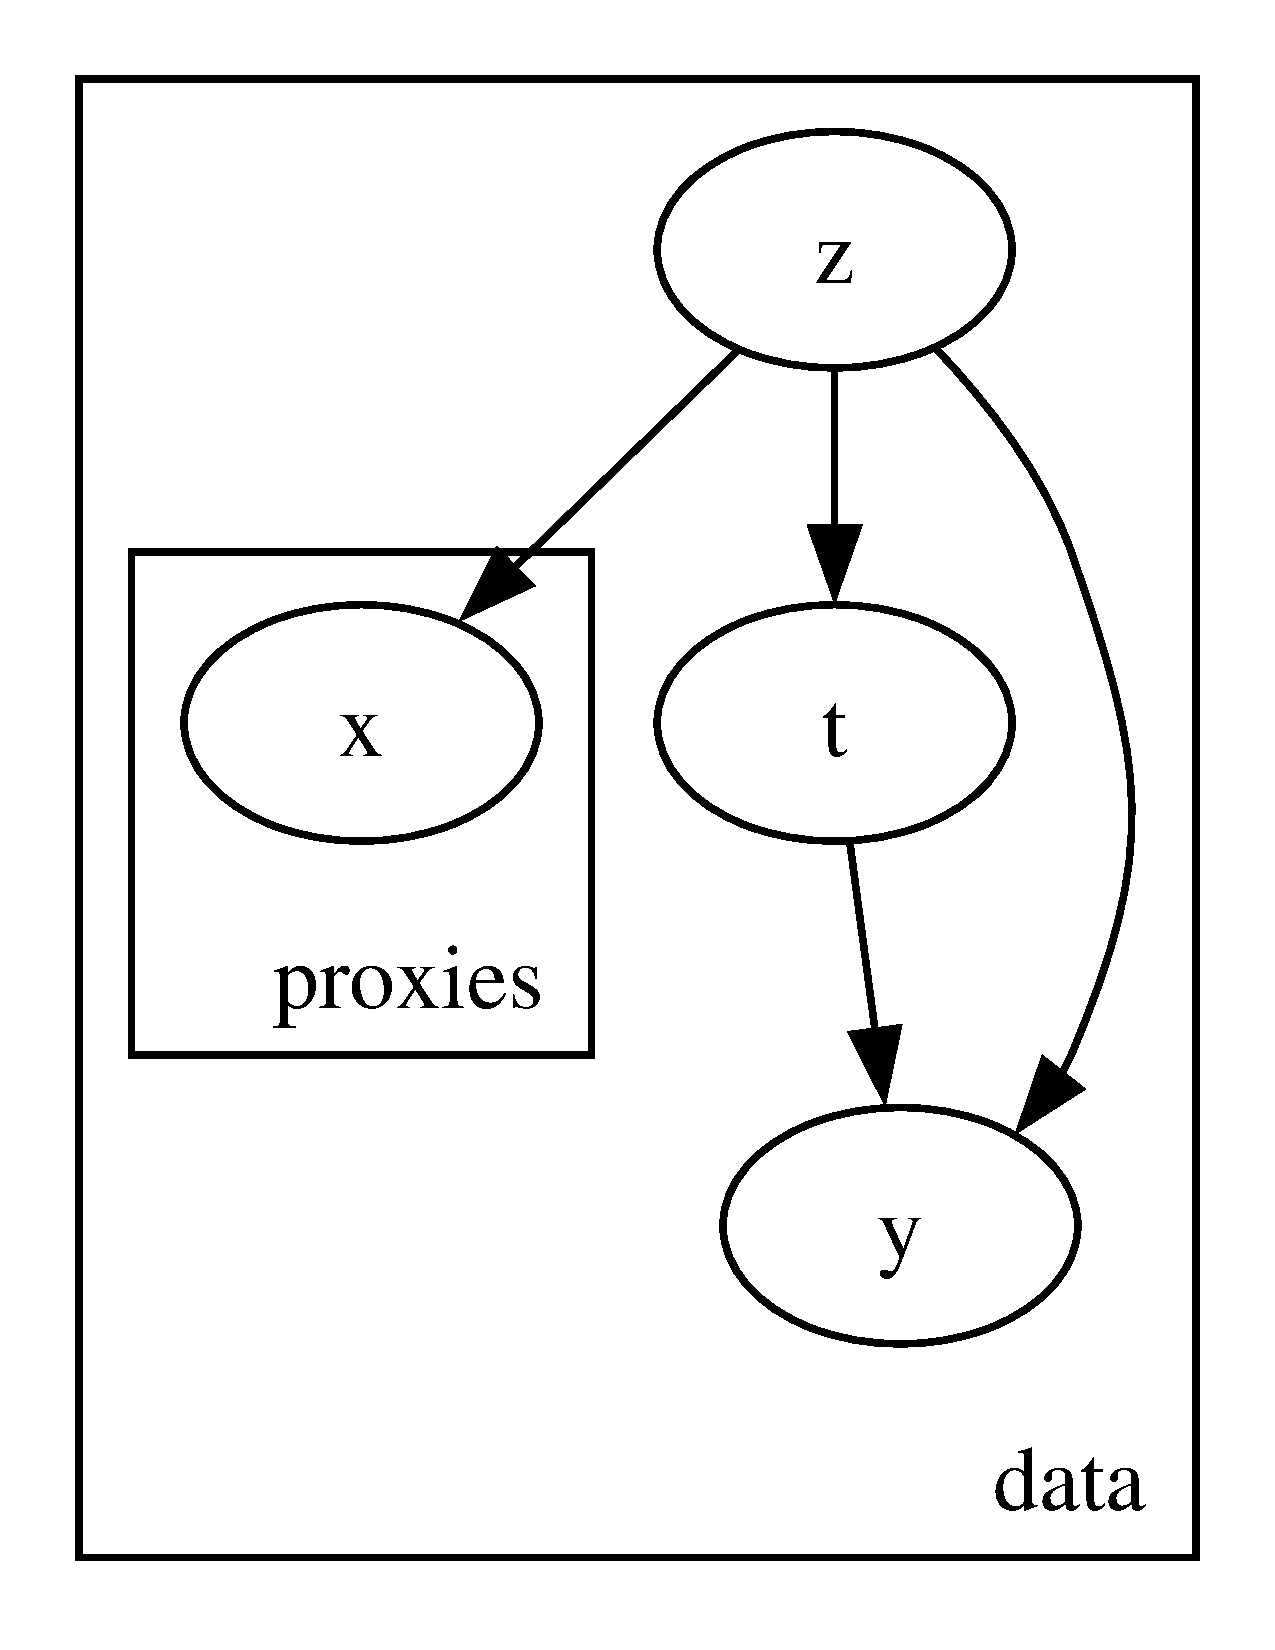
\includegraphics[width=\textwidth]{images/pyro_model.pdf}
    \end{minipage}
    \begin{minipage}{0.48\textwidth}
        \begin{equation*}
        Z \sim \mathcal{N}(0,1)
        \end{equation*}
        \begin{equation*}
             a_j \sim \mathcal{U}(-10,10)
        \end{equation*}
        \begin{equation*}
        X_j \sim \mathcal{N}(a_j z,\sigma_X^2)\,    
        \end{equation*}
        \begin{equation*}
        T | Z \sim \text{Be}(\sigma(\beta z))    
        \end{equation*}
        \small{\begin{equation*}
        Y|T,Z \sim \mathcal{N}(z + t, \sigma_Y^2)            
        \end{equation*}}
    \end{minipage}
\end{frame}

\begin{frame}{Synthetic non linear dataset}
    \begin{minipage}{0.48\textwidth}
    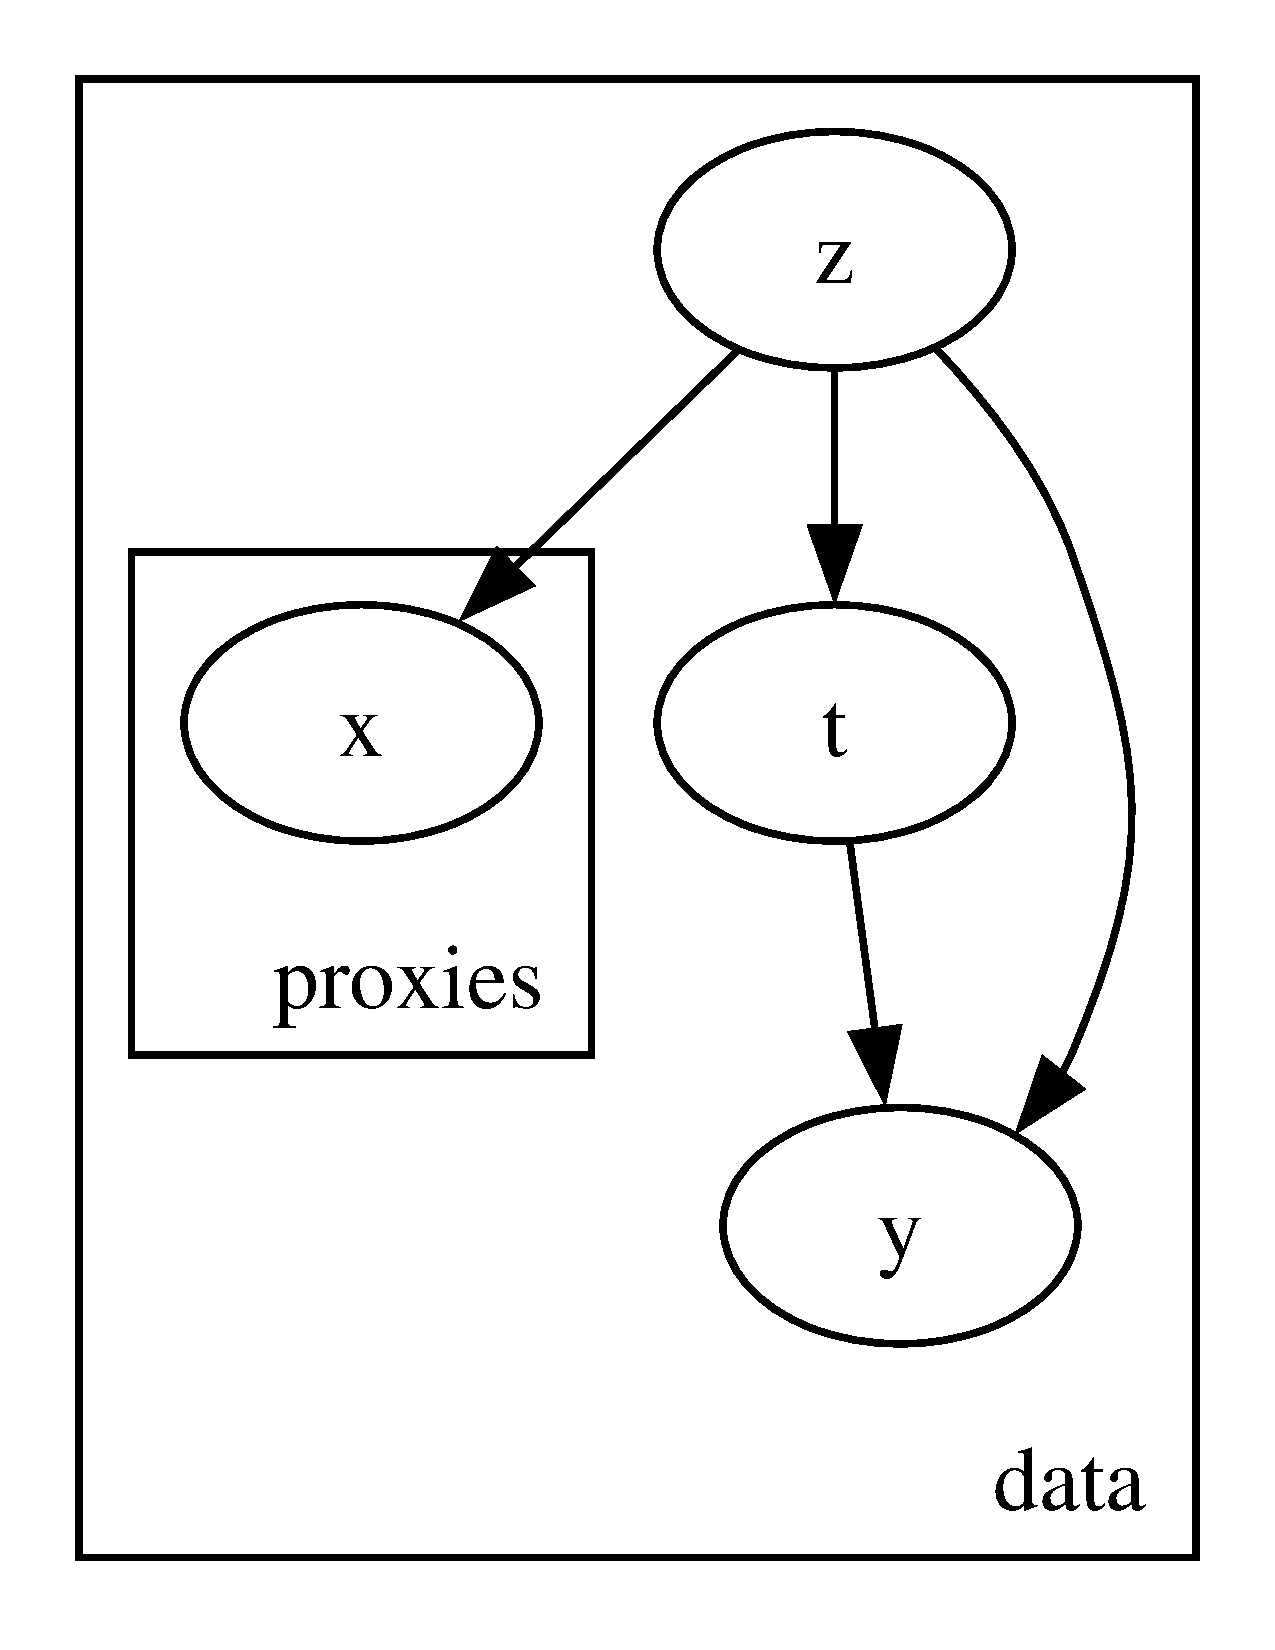
\includegraphics[width=\textwidth]{images/pyro_model.pdf}
    \end{minipage}
    \begin{minipage}{0.48\textwidth}
    \begin{equation*}
        Z \sim \mathcal{N}(0,1)
        \end{equation*}
        \begin{equation*}
            a \sim \mathcal{U}(-1.5,1.5)^d
        \end{equation*}
        \begin{equation*}
        \Sigma=\sigma_X^2[(1-\rho) \mathbb{I}+\rho J]    
        \end{equation*}
        \begin{equation*}
        X_1,...,X_d \sim \mathcal{N}(a\tanh(z),\Sigma)     
        \end{equation*}
        \begin{equation*}
        T | Z \sim \text{Be}(\sigma(\beta z))    
        \end{equation*}
\small{        \begin{equation*}
        Y|T,Z \sim \mathcal{N}\left(f_{nonLinear}(z,t),\sigma_Y^2\right)           
        \end{equation*}}
    \end{minipage}
    
\end{frame}

\begin{frame}{Experiment: latent distribution misspecified}
    
\end{frame}

\begin{frame}{Experiment: changing latent dimension}
    
\end{frame}

\begin{frame}{Experiment: increasing the treatment effect}
    
\end{frame}

\begin{frame}{Conclusions}
    
\end{frame}

{\setbeamercolor{palette primary}{fg=white, bg=bluscuro}
\begin{frame}[standout]
\thispagestyle{empty}
  {\LARGE Thank You!}
\end{frame}
}



\end{document}